\documentclass{article}
\usepackage{graphicx}
\graphicspath{ {../images/} }
\usepackage{float}
\title{CS433 Assignment 2}
\author{Shaik Awez Mehtab (23b1080)
        \\ Evuri Mohana Sreedhara Reddy (23b1017)}
\date{}
\begin{document}
    \maketitle
    Here we present the plots we have generated and our understanding of why
    they were so:
    \section*{\texttt{restartmargin}}
    \begin{figure}[H]
        \centering
        \begin{minipage}{0.45\textwidth}
            \centering
            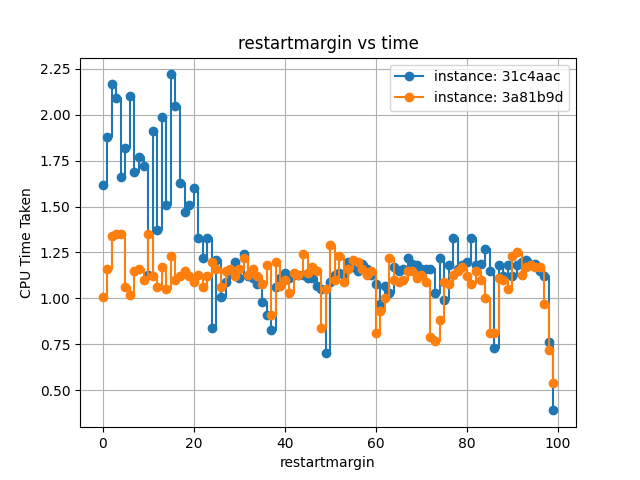
\includegraphics[width = \linewidth]{restartmargin-0.png}
        \end{minipage}
        \hfill
        \begin{minipage}{0.45\textwidth}
            \centering
            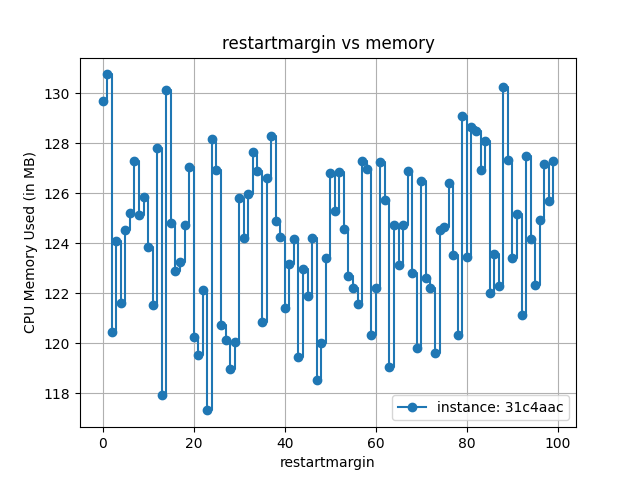
\includegraphics[width = \linewidth]{restartmargin-1.png}
        \end{minipage}
    \end{figure}

    \section*{\texttt{restartint}}
    \begin{figure}[H]
        \centering
        \begin{minipage}{0.45\textwidth}
            \centering
            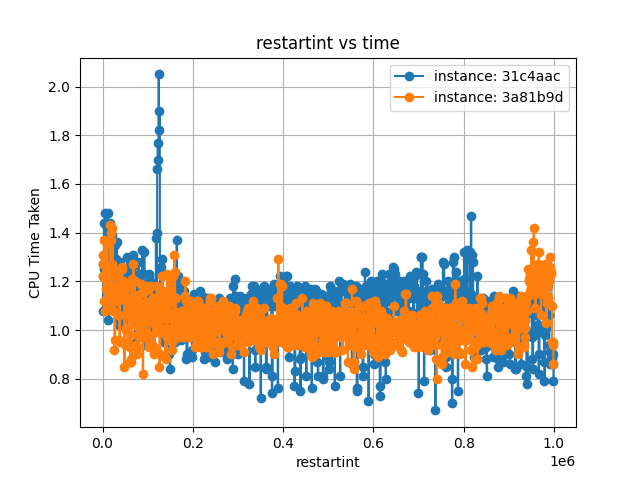
\includegraphics[width = \linewidth]{restartint-0.png}
        \end{minipage}
        \hfill
        \begin{minipage}{0.45\textwidth}
            \centering
            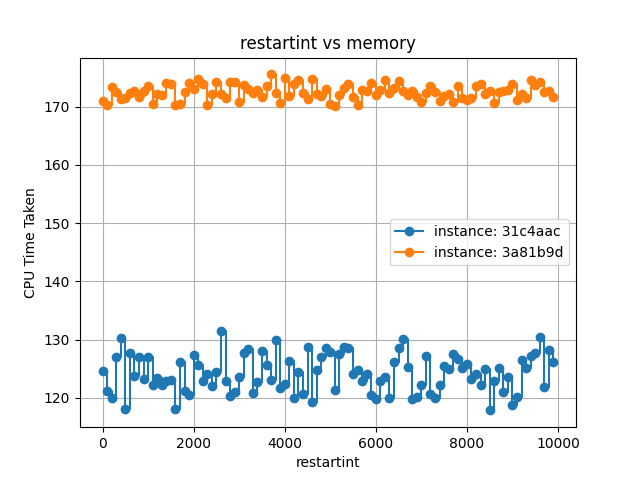
\includegraphics[width = \linewidth]{restartint-1.png}
        \end{minipage}
    \end{figure}

    \section*{\texttt{reluctant}}
    \begin{figure}[H]
        \centering
        \begin{minipage}{0.45\textwidth}
            \centering
            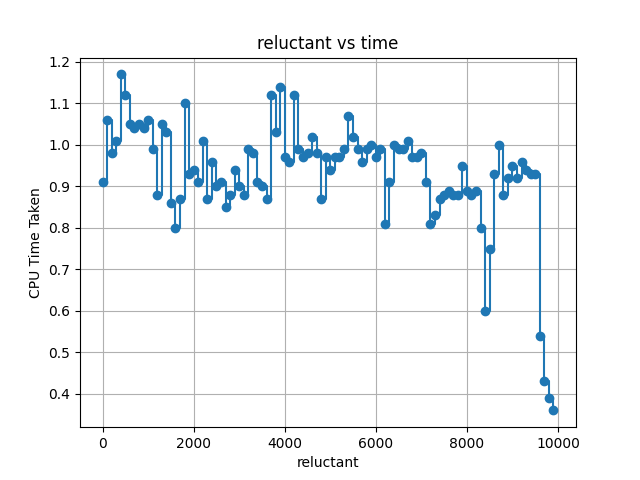
\includegraphics[width = \linewidth]{reluctant-0.png}
        \end{minipage}
        \hfill
        \begin{minipage}{0.45\textwidth}
            \centering
            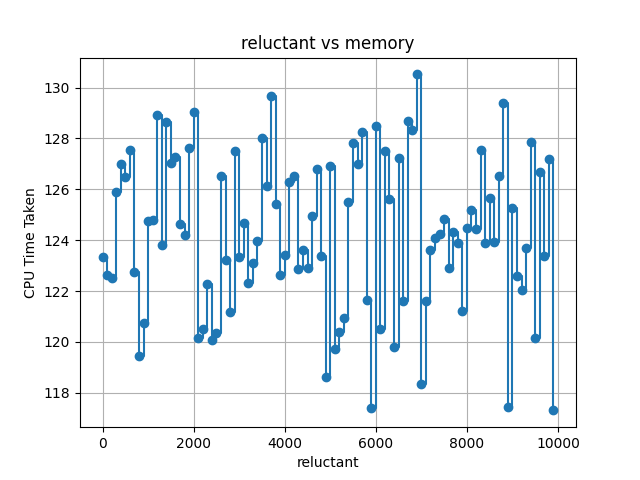
\includegraphics[width = \linewidth]{reluctant-1.png}
        \end{minipage}
    \end{figure}

    \section*{\texttt{reluctantmax}}
    \begin{figure}[H]
        \centering
        \begin{minipage}{0.45\textwidth}
            \centering
            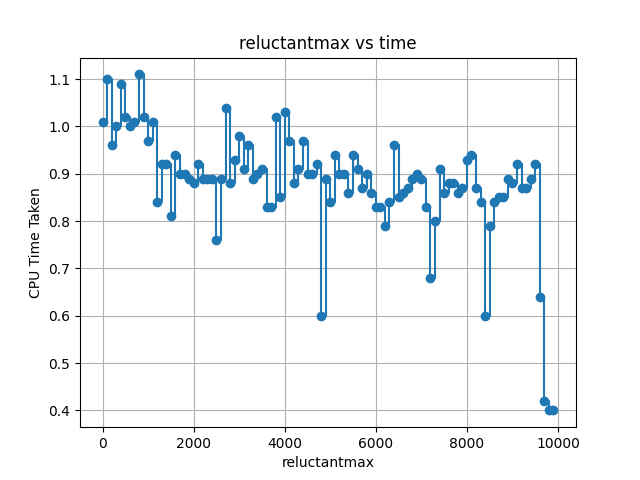
\includegraphics[width = \linewidth]{reluctantmax-0.png}
        \end{minipage}
        \hfill
        \begin{minipage}{0.45\textwidth}
            \centering
            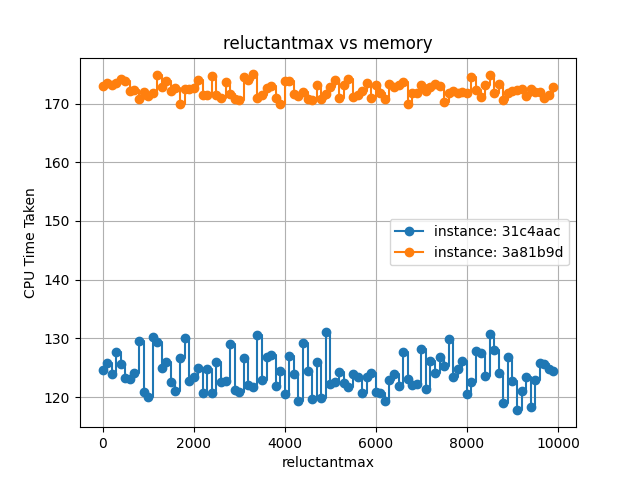
\includegraphics[width = \linewidth]{reluctantmax-1.png}
        \end{minipage}
    \end{figure}

\end{document}
